\chapter{Published models}

This chapter will present five publicly available job scheduling models based on deep reinforcement learning on graph neural networks. Three models are designed for JSSP, and two are for FJSP. For models designed for JSSP, our extension to DJSP is also presented. Each presented model is named after the GitHub repository in which it was found. 

\section{JSSP Models}

\subsection{L2D} \label{l2d_model}
\textbf{L2D} is a model published in \cite{zhang2020learning}, source code was obtained from \cite{github_l2d}. To represent the JSSP, it employs a modified disjunctive graph described in \ref{JSSP as a disjunctive graph}, where the authors start with the original disjunctive graph containing only conjunctive arcs, and after each dispatched operation, they add a conjunctive arc representing new precedence constraint between operations on the same machine. This process is shown in the Figure 3.1 below \cite{zhang2020learning}. This design solves the problem: replacing each disjunctive edge with a pair of opposite conjunctive arcs results in a fully oriented graph with too many conjunctive arcs to compute the GIN efficiently \cite{zhang2020learning}.
\par
To parametrize the policy $\pi_\theta(a_t|s_t)$, GIN for oriented graphs described in \ref{graph Isomorphism network} is used to obtain graph node embeddings $\vec{h}_o^{(K)}$ in the message passing phase. Initial node features were a 2-elementer vector $\vec{h}_o^{(0)} = (I(o), C_{LB}(o))$, where $I(o)$ is equal to 1 only if $o \in O$ is scheduled, otherwise 0, and $C_{LB}(o)$ is the lower bound of the estimated time of completion. 
\par
To select the action $a_t$ at $s_t$ in the readout phase, obtained graph embeddings are pooled using average pooling, i.e., $\vec{h}_G = \frac{1}{|O|} \sum_{o \in O} \vec{h}_o^{(K)}$, concatenated with the embedding of the eligible operation $o$ corresponding to the action $a_t$, and passed through a multi-layer perceptron to obtain a score for the corresponding action $scr(a_t) = \text{MLP}_{\pi_\theta}\left ( \left [h_o^{(T)} || h_G \right ] \right )$. The softmax function is then applied to obtain a distribution over available actions $P(a_t)$ from the scores \cite{zhang2020learning}. Selected actions are started as soon as possible. To train the policy, authors used PPO discussed in \ref{policy_optimization}.
\begin{center}
    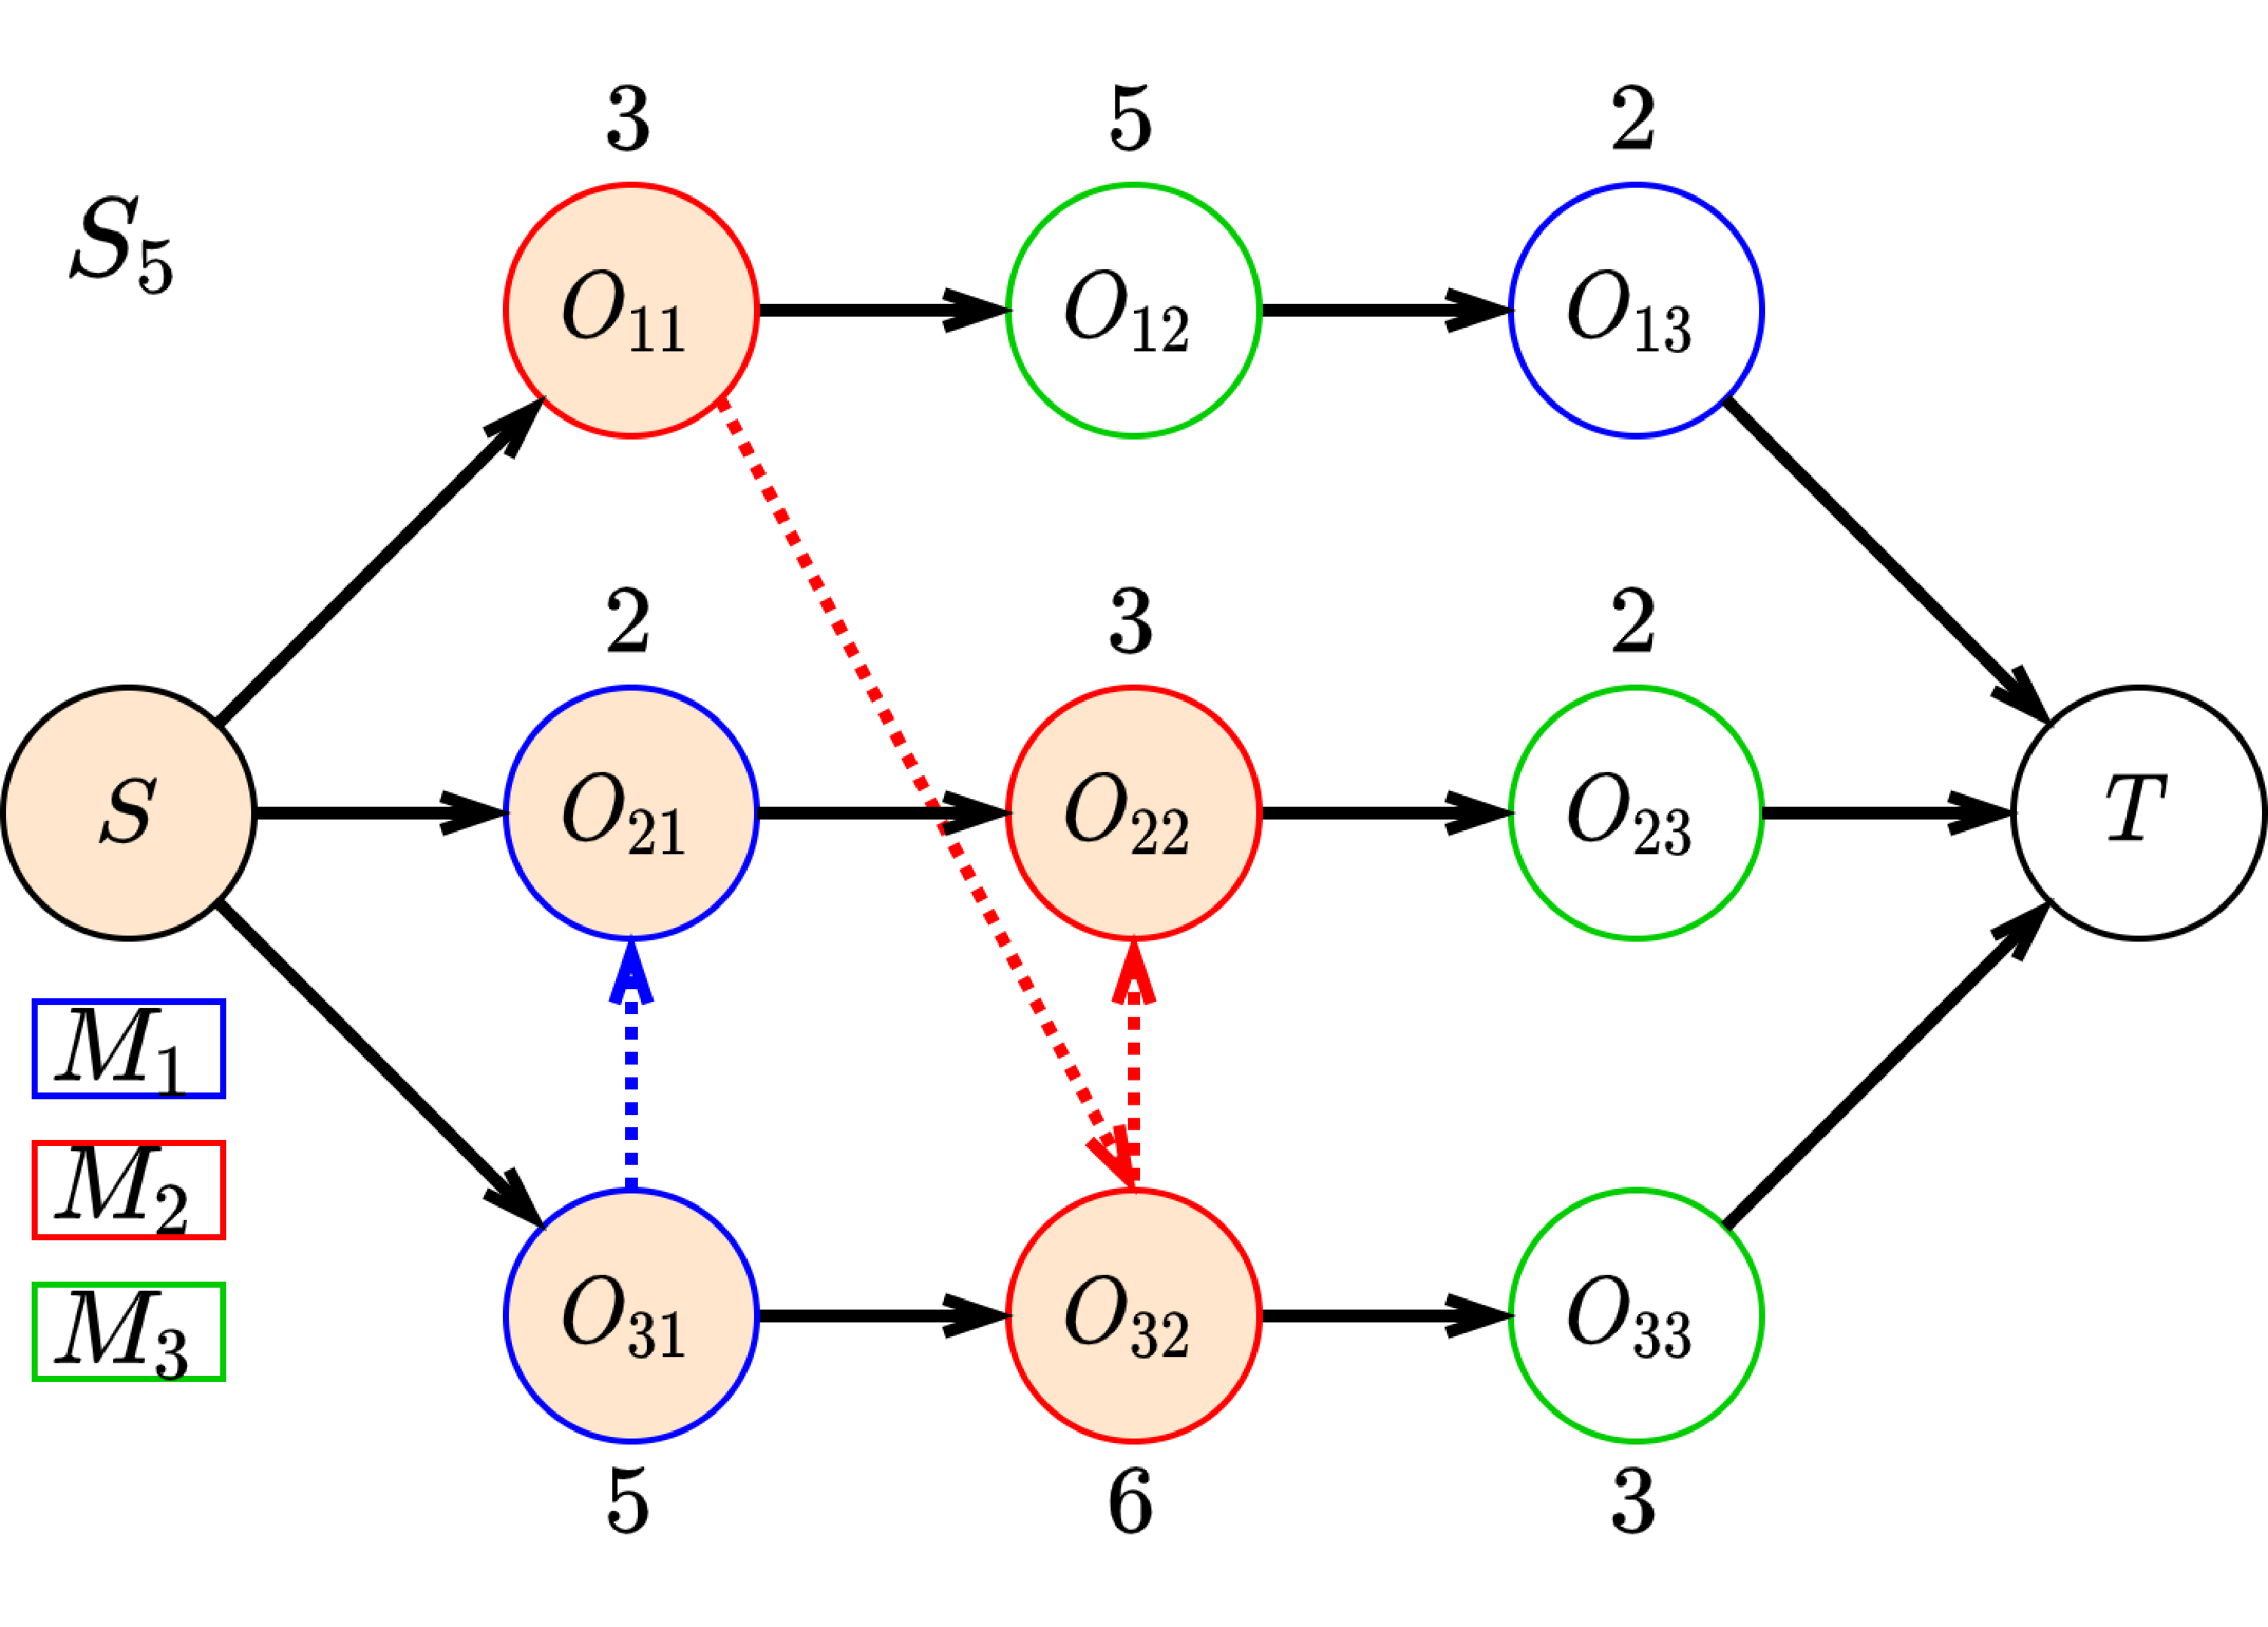
\includegraphics[width=0.75\linewidth]{images/jssp_adding_arcs.pdf}\\
    Figure 3.1: Disjunctive graph with original precedence constraints (black arrows), and three precedence constraints (red and blue arrows) between already scheduled operations (orange circles). Reproduced from \cite{zhang2020learning}.
\end{center}

\subsubsection{Dynamic L2D}

Since \textbf{L2D} is a model developed strictly for JSSP, we had to extend it to apply to DJSP. The main idea behind our algorithm is that when a new job $J_\text{new}$ arrives with the arrival time $t_a$, we want to reschedule all operations that have not started yet. To do this, we keep track of currently known jobs $J_\text{known}$, and a list of already started operations ($S_{ij} < t_a$) called \textit{plan}. When rescheduling, we first formulate the JSSP instance from known jobs and dispatch operations from the plan. By doing this, we get a partially solved JSSP with all operations with $S_{ij} \geq t_a$ removed. Then, we let \textbf{L2D} select operations to dispatch and enforce the lower bound for start time $S_{ij} \geq  t_a$. We repeat this until some termination criteria are not met; for example, no new jobs are expected to arrive. The complete algorithm written in pseudocode is shown in Algorithm \ref{algorithm:l2d}.

\begin{algorithm}
	\caption{Dynamic \textbf{L2D}} \label{algorithm:l2d}
	\begin{algorithmic}[1]
    \renewcommand{\algorithmicrequire}{\hspace*{\algorithmicindent}  \textbf{Input:}}
    \renewcommand{\algorithmicensure}{\hspace*{\algorithmicindent}  \textbf{Output:}}
    \Require Jobs known at the start $J_\text{known}$, $queue$ with arriving jobs
    \Ensure Dynamic schedule
    \State $plan \gets$ initialize empty list of actions 
    \State $instance \gets$ formulate JSSP instance from $J_\text{known}$
    \State $solution \gets$ dispatch operations in $instance$ with \textbf{L2D} 
	\While{new jobs are expected to arrive}
        \State $J_\text{new} \gets$ check if new job arrived in $queue$
        \If{$J_\text{new} = \emptyset$}
            \State \textbf{continue}
        \EndIf
        \State $t_a \gets$ arrival time of the job $J_\text{new}$
		\For{operation $O_{ij}$ in $solution$}
            \If{$S_{ij} < t_a$ and $O_{ij}$ not in $plan$}
                \State add $O_{ij}$ to the $plan$
            \EndIf
		\EndFor
        \State add $J_\text{new}$ to $J_\text{known}$
        \State $instance \gets$ formulate JSSP instance from $J_\text{known}$
        \For{operation $O_{ij}$ in $plan$}
            \State dispatch $O_{ij}$ in $instance$
        \EndFor
        \State $solution \gets$ dispatch the rest of $instance$ with \textbf{L2D} and constraint $S_{ij} \geq t_a$ 
	\EndWhile
    \State return $solution$
\end{algorithmic}
\end{algorithm}

\subsection{Wheatley}

\textbf{Wheatley} is an open-source model published in \cite{wheatley}, with source code available on GitHub \cite{github_wheatley}. It is designed not only for JSSP but also for resource-constrained project scheduling problems (RCPSPs). It has been motivated by the model \textbf{L2D} and by \cite{DBLP:journals/corr/abs-2104-03760}. It has many features beyond this thesis's scope. It supports scheduling for problems with bounded but uncertain durations and offers GNN architectures beyond those described in chapter \ref{chap:math}, e.g., Principal Neighbourhood Aggregation \cite{DBLP:journals/corr/abs-2004-05718}, Directional Graph Networks \cite{DBLP:journals/corr/abs-2010-02863}, Graph convolutional networks \cite{DBLP:journals/corr/abs-2007-02133}.
\par
JSSP is represented by a disjunctive graph described in \ref{JSSP as a disjunctive graph} with \textit{"arc adding scheme"} similar to \textbf{L2D}, i.e., it starts with the graph only containing conjunctive arcs representing precedence constraints between operations in the same job. New conjunctive arcs are added during scheduling. Node features include task completion times, a boolean feature representing if the operation has already been scheduled similarly to $I(o)$ in \textbf{L2D}, one-hot encoded machine id, a boolean feature representing if the operation is selectable. The rest can be selected from the list of options, where we selected the processing time of the operation.
\par
GNN used to obtain graph node embeddings can be chosen from multiple architectures. For this thesis, we have chosen GIN described in \ref{graph Isomorphism network} so that we can compare \textbf{Wheatley} with \textbf{L2D}. For the same reason, we have chosen average pooling after extracting the embeddings.
\par
In the readout phase, \textbf{Wheatley} passes extracted graph and node embeddings through an MLP to obtain the scores for each eligible operation.
\par
To train the agent, \textbf{Wheatley} uses the PPO algorithm discussed in \ref{policy_optimization}.

\subsubsection*{Dynamic Wheatley} \label{dynamicwheatley}
To extend Wheatley to DJSP, we consulted Wheatley's authors in the Github issue \cite{github_wheatley_djsp}. To enforce the arrival time of the job $t_a$, we were advised to add a "virtual" operation at the start of the job with processing time $t_a$ being processed by a "virtual" machine. To avoid different jobs interfering with each other, we add one "virtual" machine per one "virtual" operation.

\subsection{IEEE-ICCE-RL-JSP} \label{model_iee_icce_rl_jsp}

\textbf{IEEE-ICCE-RL-JSP} was published in \cite{10226873}, code was obtained from Github repository \cite{github_ieee_icce_rl_jsp}. Its authors represent JSSP as a heterogeneous graph discussed in \ref{FJSP as a heterogenous graph}. In each step, this model chooses one of the traditional PDRs to determine the operation to dispatch.
\par
To parametrize the policy, the authors used GIN on heterogeneous graphs discussed in \ref{graph Isomorphism network} in the message passing phase. The features of operation nodes include the status of the operation, the processing time, the remaining time of the operation, and the number of remaining operations in the current job. The features of machine nodes include the status of the corresponding machine and the remaining time of the operation being processed \cite{10226873}.
\par
In the readout phase, obtained embeddings are pooled using sum pooling and fed into a value network based on DDQN discussed in \ref{dqn}, which outputs a score value for each PDR. The agent selects a PDR with the maximum score to determine which operation to dispatch \cite{10226873}.

\subsubsection{Dynamic IEEE-ICCE-RL-JSP}

After the inspection of the source code \cite{github_ieee_icce_rl_jsp} published in \cite{10226873}, we discovered that the authors already had prepared the functionality for setting the arrival time of the job, but it was not described in the paper itself \cite{10226873}. Therefore, we only needed to modify the source code to be able to pass job arrival times to the model. 
\par
\textbf{IEEE-ICCE-RL-JSP} takes a list of jobs and their arrival times as an input. When the model chooses which operation to dispatch, operations from jobs that have not yet arrived are not listed as eligible operations, i.e., job arrival time $t_a$ is greater than the current time.

\section{FJSP Models}

\subsection{End-to-end-DRL-for-FJSP} 

\textbf{End-to-end-DRL-for-FJSP} was published in \cite{LEI2022117796}, source code was obtained from \cite{github_end_to_end_drl_for_fjsp}. The authors represented the FJSP as a disjunctive graph discussed in \ref{FJSP as a disjunctive graph}. To reduce the computational complexity, they used the \textit{"adding arc scheme"} similar to the authors of \textbf{L2D}. This process for FJSP is shown in Figure 3.2 below.
\begin{center}
    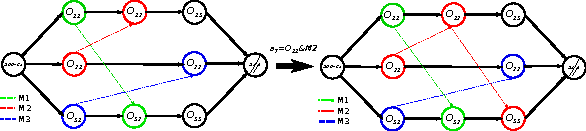
\includegraphics[width=\linewidth]{images/fjsp_adding_arcs.pdf}\\
    Figure 3.2: Action $a_7$ dispatches $O_{33}$ on $M2$ by adding a red arc corresponding to $M2$ and changing the color of $O_{33}$ to red. Reproduced from \cite{LEI2022117796}.
\end{center}
In the message passing phase, the authors use GIN, discussed in \ref{graph Isomorphism network}. Extracted operation node embeddings $\vec{h}_o^{(K)}$ are pooled using average pooling $\vec{h}_G = \frac{1}{|O|} \sum_{o \in O} \vec{h}_o^{(K)}$ as in \textbf{L2D}. The input features of each operation node are the same as in \textbf{L2D}, i.e., $\vec{h}_o^{(0)} = (I(o), C_{LB}(o))$, where $I(o)$ is equal to 1 only if $o \in O$ is scheduled, otherwise 0, and $C_{LB}(o)$ is the lower bound of the estimated time of completion.
\par
Resulting operation node embeddings do not include machine information. The authors adopt a fully connected layer to encode the state of the machine into machine embeddings $\vec{h}_m$. Those machine embeddings are then pooled to obtain a machine pooling vector $\vec{u}_m$. The input features for each machine form a vector $\vec{h}^{(0)}_k = \left ( T_k,p_{ijk}\right )$, where $T_k$ is a completion time for machine $k \in \mathcal{M}$, and $p_{ijk}$ is the processing time of operation $O_{ij}$ if its compatible with the machine $k \in \mathcal{M}$, otherwise it is an average processing time averaging over the set of compatible machines. 
\par
To select the action in the readout phase, two decoders based on multi-layer perceptrons with the same structure. Each decoder computes a probability distribution over the operation and machine space, respectively. In the first step, each decoder computes an operation score $c^o_{v}$ and machine score $c^m_{k}$ \cite{LEI2022117796}
\begin{equation}
    c^{o}_v = \text{MLP}_{\pi_{\theta}(o)} \left ( \vec{h}_v^{(K)} || \vec{h}_G || \vec{u}_m \right ) \hspace{2em} \forall v \in O \, ,
\end{equation}
\begin{equation}
    c^{m}_k = \text{MLP}_{\pi_{\theta}(m)} \left ( \vec{h}_k || \vec{h}_G || \vec{u}_m \right ) \hspace{2em} \forall k \in \mathcal{M} \, .
\end{equation}
To avoid dispatching non-eligible operations and selecting incompatible machines, their corresponding scores are set to $-\infty$ when performing operation and machine selection. Operation scores and machine scores are then normalized by a softmax function as follows \cite{LEI2022117796}
\begin{equation}
    p_i (a_o) = \frac{e^{c^o_i}}{\sum_v e^{c^o_v}} \, ,
\end{equation}
\begin{equation}
    p_j (a_m) = \frac{e^{c^m_j}}{\sum_k e^{c^m_k}} \, ,
\end{equation}
where $p_i (a_o)$ is the probability of selecting the operation $i \in O$, and $p_j (a_m)$ is the probability of selecting the machine $j \in \mathcal{M}$.\\
\par
To train the agent, the authors propose a multi-agent version of the PPO algorithm discussed in \ref{policy_optimization}. In this case, the job operation actor makes job operation action-selection using stochastic policy $\pi_{\theta_o}(a_o|s)$, and the machine actor makes machine action-selection using a stochastic policy $\pi_{\theta_m}(a_m | s, a_o)$. A single critic network with parameters $\phi$ works as an estimator to learn the approximate state-value function $\hat{v}_\phi(s)$, which is used to calculate variance-reduced advantage function estimator $\hat{A}$. The job operation/machine actor network tries to optimize loss function $L(\theta_k)$ in Algorithm \ref{algorithm:multippo}. The critic network is updated to minimize the Mean Squared Error (MSE) objective $L_\text{MSE}(\phi)$. The complete algorithm in pseudocode is in Algorithm \ref{algorithm:multippo} \cite{LEI2022117796}. On lines 3-12, two actors collect experience until all operations are scheduled and then calculate probability ratios. On lines 13-17, aggregate job operation actor, machine actor, and critic losses are calculated. Based on the losses, updates are performed $E_s$ times on lines 18-20. This whole process is repeated $E_t$ times. The multi-PPO outputs parameters of the two trained actor networks.

\begin{algorithm}
	\caption{Multi-PPO for \textbf{End-to-end-DRL-for-FJSP}} \label{algorithm:multippo}
	\begin{algorithmic}[1]
	\renewcommand{\algorithmicrequire}{\hspace*{\algorithmicindent}  \textbf{Input:}}
	\renewcommand{\algorithmicensure}{\hspace*{\algorithmicindent}  \textbf{Output:}}
	\Require Number of training steps $E_t$, PPO update steps $E_s$, batch size $B$; training actor networks $\pi_{\theta_k} (k \in \{o,m\})$, and behavior actor networks $\pi_{\theta^\text{old}_k} (k \in \{ o,m\})$ with trainable parameters $\theta_k$ and $\theta^\text{old}_k (k \in \{ o,m \})$; critic network $\hat{v}_\phi$ with trainable parameters $\phi$; policy loss coefficient $c_p$; value functon loss coefficient $c_v$; entropy loss coefficient $c_e$; clipping parameter $\epsilon$
	\Ensure Trained parameter sets $\theta_k (k \in \{ o,m \})$ of the job/machine actor
	\State Initialize $\theta_k$ and $\phi$; $\theta_k \rightarrow \theta^\text{old}_k$ 
	\For{e $=1,...,E_t$}
		\State Sampling $B$ FJSP instances from a uniform distribution;
		\For{b $=1,...,B$}
            \For{t $=0,1,2,...$}
			\State Sample $a_{b,t}^k$ based on $\pi_{\theta_{k,\text{old}}} \left( a_{b,t}^k | s_{b,t}\right)$
			\State Observe reward $r_{b,t}$ and next state $s_{b,t+1}$;
			\State $\hat{A}_{b,t} = \sum_{t'=t}^T\gamma^{t'}r_{b,t'} - \hat{v}_\phi(s_{b,t}); \delta_{b,t}^k(\theta_k) = \frac{\pi_{\theta_k}\left(a^k_{b,t} | s_{b,t}\right)}{\pi_{\theta_{k,\text{old}}}\left(a^k_{b,t} | s_{b,t}\right)}$;
            \If{$s_{b,t}$ is terminal}
                \State break;
            \EndIf
            \EndFor
        \State $L_{CLIP}^{b,k}(\theta_k) = \mathbb{E} \left [ \min \{\delta_{b,t}^k(\theta_k)\hat{A}_{b,t}, \text{clip}\left( \delta_{b,t}^k(\theta_k), 1-\epsilon, 1+\epsilon\right) \hat{A}_{b,t} \} \right ]$
        \State $L_E^{b,k}(\theta_k) = \mathbb{E} \left [ \text{Entropy}\left(\pi_{\theta_k}\left(a_{b,t}^k | s_{b,t}\right)\right)\right ]$
        \State Aggregate job/machine actors Loss: $L(\theta_k) = c_p L_\text{CLIP}^{b,k}(\theta_k) + c_e L_e^{b,k}(\theta_k)$
        \State Aggregate critic Loss: $L_\text{MSE}(\phi)=(r_t, \hat{v}_\phi(s_t))$
		\EndFor
    \For{$PPO$ step $=1,...,E_s$}
        \State Update $\theta_k$ by a gradient method w.r.t. $L(\theta_k)$ 
        \State Update $\phi$ by a gradient method w.r.t. $L_\text{MSE}(\phi)$
    \EndFor
    \State $\theta_k^\text{old} \gets \theta_k$
	\EndFor
	\State return $\theta_k$
\end{algorithmic}
\end{algorithm}

\subsection{fjsp-drl} \label{model_fjsp_drl}

The model \textbf{fjsp-drl} was published in \cite{9826438}, and the source code was obtained from \cite{github_fjsp_drl}.
\par
The authors represented FJSP as a heterogeneous graph discussed in \ref{FJSP as a heterogenous graph}. They propose a two-stage embedding process to extract node embeddings in the message-passing phase called Heterogeneous Graph Neural Network (HGNN). In the first stage, using GIN discussed in \ref{graph Isomorphism network}, machine embeddings $\vec{\nu}_l^{(k)}$ are updated by aggregating the information from its neighborhood. Operation embeddings $\vec{\mu}_{ij}^{(k)}$ of operation $O_{ij} \in \mathcal{N}(M_l)$ are concatenated with edge embeddings $\vec{\lambda}_{ijl}^{(k)}$ of the corresponding $O-M$ edge connecting machine $M_l$ and operation $O_{ij}$ to obtain $\vec{\mu}_{ijl}^{(k)} = \left [ \vec{\mu}_{ij}^{(k)}||\vec{\lambda}_{ijl}\right ]$. Authors use two shared linear transformations $\boldsymbol{W}^M$ and $\boldsymbol{W}^O$ for machines and operations, respectively, to calculate attention coefficients $e_{ijl}$ as follows \cite{9826438}
\begin{equation}
    e_{ijl} = \text{LeakyRelu}\left (\vec{b} \cdot \left [ \boldsymbol{W}^M \vec{\nu}_l^{(k)} || \boldsymbol{W}^O \vec{\mu}_{ijl}^{(k)} \right ]\right ) \, .
\end{equation}
Attention coefficient $e_{ll}$ of the machine $M_l$ to itself is calculated as follows \cite{9826438}
\begin{equation}
    e_{ll} = \text{LeakyRelu}\left (\vec{b} \cdot \left [ \boldsymbol{W}^M \vec{\nu}_l^{(k)} || \boldsymbol{W}^M \vec{\nu}_l^{(k)} \right ]\right ) \, .
\end{equation}
Then, all attention coefficients $e_{ijl}$ and $e_{ll}$ are normalized using the Softmax function to get normalized attention coefficients $\alpha_{ijl}$ and $\alpha_{ll}$. New embeddings are then calculated as follows \cite{9826438}
\begin{equation}
    \vec{\nu}_l^{(k+1)} = \sigma \left ( \alpha_{ll} \boldsymbol{W}^M \vec{\nu}_l^{(k)} + \sum_{O_{ij} \in \mathcal{N}(M_l)} \alpha_{ijk} \boldsymbol{W}^O\vec{\mu}_{ijl}^{(k)}\right ) \hspace{2em} \forall M_l \in M
\end{equation}
\par
In the second stage, to update operation node embeddings, authors use five MLPs (denoted as $\text{MLP}_{\theta_i}$ for the i-th MLP). Individual MLPs are used to process embeddings of a preceding operation $\vec{\mu}_{i,j-1}^{(k)}$, succeeding operation $\vec{\mu}_{i,j+1}^{(k)}$, embedding of the operation itself $\vec{\mu}_{ij}^{(k)}$, and aggregated neighboring machine embedding $\nu_{ij}^{(k+1)} = \sum_{M_l\in\mathcal{N}(O_{ij})} \vec{\nu}_l^{(k+1)}$. Operation embedding update is then performed as follows \cite{9826438}
\begin{equation}
    \begin{split}
        \mu_{ij}^{(k+1)}  = \text{MLP}_{\theta_0} \Bigg( 
            &\text{ELU} \Big[ 
                \text{MLP}_{\theta_1}\left(\vec{\mu}_{i,j-1}^{(k)}\right) || 
                \text{MLP}_{\theta_2}\left(\vec{\mu}_{i,j+1}^{(k)}\right) || \\
                &\text{MLP}_{\theta_3}\left(\vec{\nu}_{ij}^{(k+1)}\right) || 
                \text{MLP}_{\theta_4}\left(\vec{\mu}_{ij}^{(k)}\right)
            \Big]    
        \Bigg) \, ,
\end{split}
\end{equation}
where ELU is the Exponential Linear Unit function with parameter $\alpha > 0$ defined as \cite{elu_activation} 
\begin{equation}
    \text{ELU}(x) = \begin{cases} x & \mbox{if } x > 0 \\ \alpha (\exp(x) - 1) & \mbox{if } x \leq 0 \end{cases} \, .
\end{equation}
\par
This two-stage embedding process can be thought of as one HGNN step (layer). After K steps, the final machine embeddings $\vec{\nu}_k^{(K)}$ and operation node embeddings $\vec{\mu}_{ij}^{(K)}$ are mean-pooled and concatenated. The final vector $\vec{h}_H$ is the embedding of the heterogeneous graph $H$ \cite{9826438}
\begin{equation}
    \vec{h}_H = 
        \left [
            \frac{1}{|O|}\sum_{O_{ij} \in O} \vec{\mu}_{ij}^{(K)} 
            \middle\| 
            \frac{1}{|M|}\sum_{M_k \in M} \vec{\nu}_k^{(K)}
        \right ] \, .
\end{equation}
In the readout phase, for each feasible action $a_t = (O_{ij}, M_l) \in A_t$ in state $s_t$ at step $t$, the corresponding operation node and machine embeddings are concatenated with heterogeneous graph embedding and fed into an MLP with parameters $\omega$ with a tanh activation to get the priority index \cite{9826438}
\begin{equation}
    P(a_t, s_t) = \text{MLP}_{\omega} \left [ \vec{\mu}_{ij}^{(K)} || \vec{\nu}_l^{(K)} || \vec{h}_H \right ] \, .
\end{equation}
The probability of selection action $a_t$ is obtained by applying softmax over all possible actions
\begin{equation}
    \pi_\omega (a_t|s_t) = \frac{\exp{P(a_t,s_t)}}{\sum_{a_t'\in A_t}\exp(P(a_t',s_t))} \hspace{2em} \forall a_t \in A_t \, . 
\end{equation}
Initial operation node features $\vec{\mu}_{ij}^{(0)}$ include \cite{9826438}
\begin{enumerate}
    \item  binary value indicating whether the operation has been scheduled
    \item number of neighboring machines $|\mathcal{O}_{ij}|$
    \item processing time $p_{ijk}$ if $O_{ij}$ is scheduled, otherwise $\overline{p}_{ij} = \frac{1}{|\mathcal{O_{ij}}|}\sum_k p_{ijk}$
    \item estimated or actual start time of $O_{ij}$ in the corresponding partial schedule $S_{ij}(t)$
    \item number of unscheduled operations in the job
    \item job completion time in the partial schedule $S(t)$
\end{enumerate}
\clearpage
Initial machine node features $\vec{\nu}_{l}^{(0)}$ include \cite{9826438}
\begin{enumerate}
    \item available time: time when machine $M_l$ will finish all its currently assigned operations
    \item number of neighboring operations $|\mathcal{N}(M_l)|$
    \item utilization: ratio of nonidle time to the to the total production time
\end{enumerate}
Initial $O-M$ arc features $\vec{\lambda}_{ijl}^{(0)}$ include only corresponding processing time $p_{ijl}$ \cite{9826438}.
\par
The authors used a modified version of the PPO discussed in section \ref{policy_optimization} to train the agent. The actor is the policy network $\pi_\omega$, and critic $v_\phi$ is the network that takes $h_H$ computed by HGNN as an input and predicts the value $v(s_t)$. The critic has the same structure as the actor but has a different number of inputs. The full algorithm is written in pseudocode in Algorithm \ref{algorithm:hgnnppo}. 

\begin{algorithm}
	\caption{HGNN Training procedure with PPO for \textbf{fjsp-drl}} \label{algorithm:hgnnppo}
	\begin{algorithmic}[1]
	\renewcommand{\algorithmicrequire}{\hspace*{\algorithmicindent}  \textbf{Input:}}
	\renewcommand{\algorithmicensure}{\hspace*{\algorithmicindent}  \textbf{Output:}}
	\Require HGNN network, policy network and critic network with trainable parameters $\theta$, $\omega$ and $\phi$
	\Ensure Trained parameters
	\State Sample a batch of $B$ FJSP instances
	\For{iter $=1,2,...,I$}
		\For{b $=1,2,...,B$}  \Comment{In parallel}
			\State Initialize $s_t$ based on instance $b$
            \While{$s_t$ is not terminal}
                \State Extract embeddings using HGNN
                \State Sample $a_t \sim \pi_\omega(\cdot | s_t)$
                \State Receive reward $r_t$ and next state $s_{t+1}$
                \State $s_t \gets s_{t+1}$
            \EndWhile
			\State Compute the generalised advantage estimates $\hat{A_t}$ for each step
        \State Compute  the PPO loss $L$, and optimize the parameters $\theta$, $\omega$, and $\phi$
        \State Update network parameters
        \State Validate the policy every 10 iterations
        \State Sample a new batch of $B$ FJSP instances every 20 iterations
		\EndFor
	\EndFor
	\State return $\theta_k$
\end{algorithmic}
\end{algorithm}